\documentclass[main]{subfiles}

\begin{document}

\begin{figure}[!ht]
  \centering
  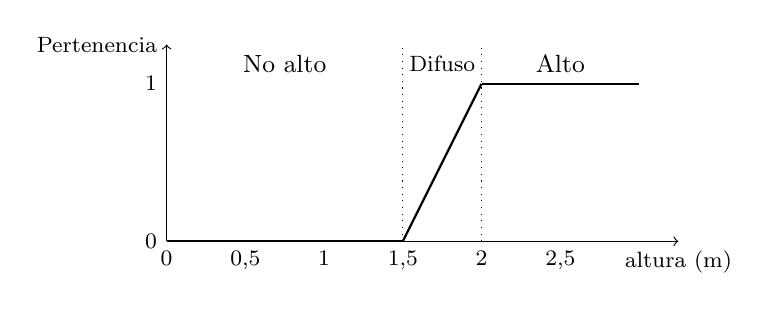
\begin{tikzpicture}

  % horizontal axis
  \draw[->] (0,0) -- (6.5,0) node[anchor=north] {\footnotesize altura (m)};
  % labels
  \draw	(0,0) node[anchor=north] {\footnotesize 0}
  		(1,0) node[anchor=north] {\footnotesize 0,5}
  		(2,0) node[anchor=north] {\footnotesize 1}
  		(3,0) node[anchor=north] {\footnotesize 1,5}
  		(4,0) node[anchor=north] {\footnotesize 2}
  		(5,0) node[anchor=north] {\footnotesize 2,5};

  % vertical axis
  \draw[->] (0,0) -- (0,2.5) node[anchor=east] {\footnotesize Pertenencia};
  % labels
  \draw	(0,0) node[anchor=east] {\footnotesize 0}
  		(0,2) node[anchor=east] {\footnotesize 1};

  % funcion
  \draw[thick] (0,0)--(3,0);
  \draw[thick] (3,0)--(4,2);
  \draw[thick] (4,2)--(6,2);
  \draw[dotted] (3,0)--(3,2.5);
  \draw[dotted] (4,0)--(4,2.5);
  \draw (5,2.25) node {\small Alto}; %label
  \draw (3.5,2.25) node {\footnotesize Difuso}; %label
  \draw (1.5,2.25) node {\small No alto}; %label



  \end{tikzpicture}
  \caption{Representación de la pertenencia de los elementos para la lógica difusa. \label{fig:altodifusa}}
\end{figure}

\end{document}
